\documentclass[12pt]{article}

\usepackage{lmodern}
\usepackage[T1]{fontenc}
\usepackage[spanish,activeacute]{babel}
\usepackage{mathtools}
\usepackage{graphicx}
\usepackage{geometry,pdfpages}
\usepackage{wrapfig}
\usepackage{enumerate} 
\usepackage{parskip}


\geometry{
	letterpaper,%showframe,
	left=30mm,top=10mm,right=30mm,bottom=10mm,
	headheight=6mm,headsep=7mm,foot=5mm,footskip=15mm,
	includeheadfoot
}

\setlength{\parindent}{0cm}


\begin{document}

		
	\begin{wrapfigure}[0]{r}{0.15\textwidth}
		\vspace{-142pt}
		
\includegraphics[width=2cm]{loguito}
	\end{wrapfigure}
	
	\begin{center}
		\fbox{\parbox[t]{\linewidth}{
				\begin{flushleft}
					Universidad Centroamericana "Jos'e Sime'on Cañas" \linebreak
					Facultad de Ingenier'ia y Arquitectura\linebreak
					Departamento de Electr'onica e Inform'atica\linebreak
					\textbf{Materia: }An'alisis Num'erico\linebreak
					\textbf{Catedr'atico: } Daniel Sosa\linebreak
					\textbf{Instructor: } Kevin Lopez\linebreak
					\textbf{Estudiante: } Elsy Alejandra Chavez Mendoza ($\texttt{00125717}$)\linebreak
					\textbf{Estudiante: } Fredy Alexander Sanchez Perez ($\texttt{00082817}$)\linebreak
					\textbf{Estudiante: } Erick Fernando Leones Arevalo ($\texttt{00092217}$)\linebreak
					\textbf{Estudiante: } German Alexander Castro Portillo ($\texttt{00229017}$)\linebreak
					Viernes 28 de junio de 2019
				\end{flushleft}
		}}
	\end{center}
	
		\section*{Definiciones}
			El m'etodo de cuadratura de Gauss es un m'etodo num'erico para evaluar integrales definidas de funciones, por medio de sumatorias f'aciles de implementar, de la siguiente forma:
			
			\begin{equation}\label{eq:eq1}
			\int_{a}^{b} f(x) \cdot dx \approx \sum_{i=1}^{n} c_{i} f(x_{i}) \approx w_{1}f(x_{1})+w_{2}f(x_{2})+w_{3}f(x_{3})+...+w_{n}f(x_{n})
			\end{equation}
			
			Donde $\mathrm{w_{i}}$ se refiere a los pesos o coeficientes que en el caso de cuadratura de Gauss se explicar'a c'omo calcularse m'as adelante.
			Y donde $\mathrm{x_{i}}$ se refiere a las ra'ices de la funci'on como polinomio lo cual recordando se obtienen igualando la funci'on a cero, es decir:
			\begin{equation}\label{eq:eq2}
				f(x)=0
			\end{equation}
			
			Y los resultados obtenidos siguientes $\mathrm{x_{1}, x_{2},..., x_{n}}$ son las ra'ices de la funci'on.
			
			Para este m'etodo tambi'en debemos recordar la f'ormula del polinomio interpolante de Legendre el cual es:
			\begin{equation}\label{eq:eq3}
				\sum_{i=1}^{n}L_{i}(x)f(x_{i})
			\end{equation} 
			Donde:
			\begin{equation}
				L_{i}(x)=\prod_{j=1}^{n}\frac{x - x_{j}}{x_{i} - x_{j}}
			\end{equation}
			
			Tambi'en para contextualizar, recordemos de los otros m'etodos de cuadratura que, la regla del trapecio (Newton-Cotes para $\mathrm{n=1}$) tiene grado de precisi'on uno. La regla de Simpson ($\mathrm{n=2}$) es correcta hasta los polinomios de tercer grado inclusive. A diferencia de Newton Cotes la cuadratura de Gauss posee un grado de precisi'on de $\mathrm{2_{n}-1}$, adem'as que selecciona los puntos de evaluaci'on de manera 'optima y no de forma igualmente espaciada como lo hacen las f'ormulas de Newton-Cotes.
				
			
		\section*{Resultados te'oricos}
			\subsection*{Polinomios Ortogonales}
				Antes de explicar la cuadratura gaussiana se debe conocer acerca de lo que son los polinomios ortogonales para luego proceder a utilizar el polinomio de Legendre.
				El conjunto de funciones diferentes de cero $\mathrm{\lbrace p_{0}, ..., p_{n}\rbrace}$ en el intervalo $\mathrm{[a,b]}$ es ortogonal en $\mathrm{[a,b]}$ si
				\begin{equation}
					\int_{a}^{b}p_{j}(x)p_{k}(x)\cdot dx = \left\{\begin{array}{lcc}
						0 & j\ne k\\
						\ne 0 & j=k
					\end{array}
					\right.	
				\end{equation}
				
				\subsection*{Polinomios de Legendre}
					Conociendo acerca de los polinomios ortogonales, ahora se da a conocer acerca de un conjunto de este tipo de polinomios llamado de Legendre los cuales son ortogonales en el intervalo $\mathrm{[-1, 1]}$ y se obtienen de la siguiente f'ormula:		
					\begin{equation}
						p_{i}(x)=\frac{1}{2^{i}i!}\frac{d^{i}}{d x^{i}}[(x^{2}-1)^{i}]
					\end{equation}
					Cuya demostraci'on omitimos.
					
					Existe un m'etodo por el cual se puede determinar los nodos y coeficientes  para las f'ormulas que dan el resultado exacto de los polinomios de grado superior. Se consideran varias colecciones de polinomios ortogonales, los cuales son funciones que tienen la propiedad de que una integral definida del producto de dos de ellos es igual a cero. Esta colecci'on de polinomios son llamados polinomios de Legendre, que van desde $\mathrm{P_{0}}$ hasta $\mathrm{P_{n}}$ y tienen las propiedades:
					\begin{enumerate}[1.]
						\item 
						Para cada $\mathrm{n}$, $\mathrm{P_{n}(x)}$ es un polinomio m'onico (polinomio de una variable cuyo coeficiente principal es 1) con grado $n$.
						\item
						$\mathrm{\int_{-1}^{1}P(x)P_{n}(x)\cdot dx = 0}$ cuando $\mathrm{P(x)}$ sea un polinomio de grado menor a $\mathrm{n}$.
					\end{enumerate}
					
					Los primeros polinomios de Legendre son:\\
					$\mathrm{P_{0}(x)=1}$\\
					$\mathrm{P_{1}(x)=1}$\\
					$\mathrm{P_{2}(x)=x^{2}-\frac{3}{5}x}$\\
					$\mathrm{P_{3}(x)=x^{3}-\frac{6}{7}x^{2}+\frac{3}{35}}$\\	
				\subsection*{F'ormula de la Cuadratura Gaussiana}
					\begin{equation}
						\int_{-1}^{1}f(x)\approx \sum_{i=1}^{n}c_{i}f(x_{i})
					\end{equation}
					Los nodos o ra'ices $\mathrm{x_{1}, x_{2}, ..., x_{n}}$ en el intervalo $\mathrm{[-1,1]}$ y los coeficientes $\mathrm{c_{1}, c_{2}, ..., c_{n}}$, son elegidos para minimizar el error obtenido en la aproximaci'on.
					
					Para el caso de las ra'ices $\mathrm{x_{i}}$ se utiliza el polinomio de Legendre del grado que se desee evaluar y se obtienen las ra'ices de este, las cuales se utilizan en la formula de Gauss y luego para el caso de los coeficientes $\mathrm{c_{i}}$ se obtienen de la misma forma que en Lagrange se obtiene el $\mathrm{L_{i}(x)}$ siendo $\mathrm{x_{i}}$ de esta f'ormula las ra'ices calculadas con el polinomio de Legendre.
					
					Veamos el siguiente ejemplo:\\
					Polinomio:  $\mathrm{P_{2}(x)=x^{2}-\frac{1}{3}}$\\
					Se obtienen las ra'ices:
					\begin{equation}
						\begin{array}{lcc}
							x^{2}-\frac{1}{3}=0\\
							\\
							x^{2}=\frac{1}{3}\\
							x=\pm \sqrt{\frac{1}{3}}\left\{\begin{array}{lcc}
							x_{1}=\sqrt{\frac{1}{3}}\\
							x_{2}=-\sqrt{\frac{1}{3}}
							\end{array} 
							\right.
						\end{array}
					\end{equation}
					Se procede ahora a obtener los coeficientes:
					\begin{equation}
						c_{1}=\int_{-1}^{1}\frac{(x-x_{2})}{(x_{1}-x_{2})}\cdot dx=\int_{-1}^{1}\frac{x-(-\sqrt{\frac{1}{3}})}{\sqrt{\frac{1}{3}}-(-\sqrt{\frac{1}{3}})}\cdot dx=1
					\end{equation}
					\begin{equation}
					c_{2}=\int_{-1}^{1}\frac{(x-x_{1})}{(x_{2}-x_{1})}\cdot dx=\int_{-1}^{1}\frac{x-\sqrt{\frac{1}{3}}}{-\sqrt{\frac{1}{3}}-\sqrt{\frac{1}{3}}}\cdot dx=1
					\end{equation}
					Y es as'i como se obtienen los siguientes resultados para los diferentes grados que se eval'uen.
				\begin{center}
					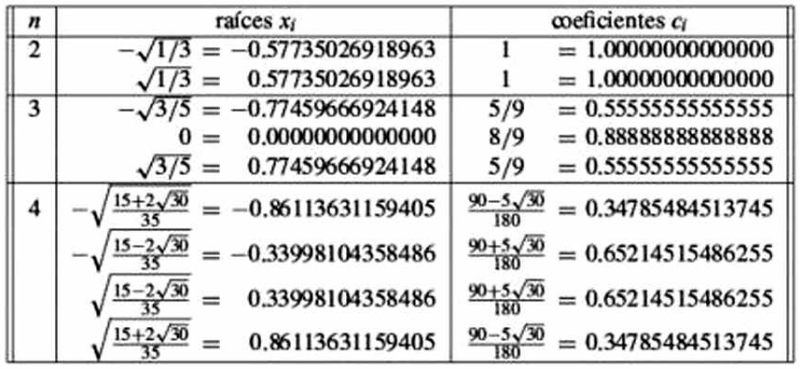
\includegraphics[width=15cm]{roots}
					\par
					\vspace{0.2cm}
					ra'ices $\mathrm{x_{i}}$ de los n-'esimos polinomios de Legendre y coeficientes $\mathrm{c_{i}}$
				\end{center}
				
				Fig 1. Para aproximar las integrales en un intervalo general $[a, b]$, el problema debe trasladarse de nuevo a $[-1, 1]$ . Si se usa la sustituci'on $\mathrm{t= \frac{(2x-a-b)}{(b-a)}}$ la nueva f'ormula queda de la siguiente manera:
				\begin{equation}
					\int_{a}^{b}f(x)=\int_{-1}^{1}f(\frac{(b-a)t+b+a}{2})\frac{b-a}{2}\cdot dt
				\end{equation}
		\section*{Resultados pr'acticos}
			Ejemplo de uso de cuadratura gaussiana:
			\begin{equation}
				\int_{-1}^{1}(x^{4})\cdot dx
			\end{equation}
			Calculando el valor correcto:
			\begin{equation}
			\int_{-1}^{1}(x^{4})\cdot dx=\frac{2}{5}=0.4
			\end{equation}
			Calculando el valor aproximado utilizando la cuadratura gaussiana para $\mathrm{n=2}$:
			\begin{equation}
				\begin{array}{lcc}
					\int_{-1}^{1}f(x)\approx \sum_{i=1}^{n}c_{i}f(x_{i})\\
					\\
					\sum_{i=1}^{n}c_{i}f(x_{i})=c_{1}f(x_{1})+c_{2}f(x_{2})\\
					\\
					((-\sqrt{\frac{1}{3}})^{4}+(\sqrt{\frac{1}{3}})^{4})=0.22222222222222868
				\end{array}
			\end{equation}
			Calculando el valor aproximado utilizando la cuadratura gaussiana para $\mathrm{n=3}$:
			\begin{equation}
			\begin{array}{lcc}
			\int_{-1}^{1}f(x)\approx \sum_{i=1}^{n}c_{i}f(x_{i})\\
			\\
			\sum_{i=1}^{n}c_{i}f(x_{i})=c_{1}f(x_{1})+c_{2}f(x_{2})+c_{3}f(x_{3})\\
			\\
			\frac{5}{9}(-\sqrt{\frac{3}{5}})^{4}+\frac{8}{9}(0)^{4}+\frac{5}{9}(\sqrt{\frac{3}{5}})^{4}=0.399999999999989
			\end{array}
			\end{equation}
			Calculando el valor aproximado utilizando la cuadratura gaussiana para $\mathrm{n=4}$:
			\begin{equation}
			\begin{array}{lcc}
			\int_{-1}^{1}f(x)\approx \sum_{i=1}^{n}c_{i}f(x_{i})\\
			\\
			\sum_{i=1}^{n}c_{i}f(x_{i})=c_{1}f(x_{1})+c_{2}f(x_{2})+c_{3}f(x_{3})+c_{4}f(x_{4})\\
			\\
			\frac{90-5\sqrt{30}}{180}[(-\sqrt{\frac{15+2\sqrt{30}}{35}})^{4}+(\sqrt{\frac{15+2\sqrt{30}}{35}})^{4}]+\frac{90+5\sqrt{30}}{180}[(-\sqrt{\frac{15+2\sqrt{30}}{35}})^{4}+(\sqrt{\frac{15+2\sqrt{30}}{35}})^{4}]=0.3999999999999921
			\end{array}
			\end{equation}
			
			Ejemplo de cambio de intervalos a $[-1,1]$:
			\begin{equation}
				\int_{0}^{4}\frac{x}{\sqrt{x^{2}+9}}\cdot dx
			\end{equation}
			Calculando el valor correcto:
			\begin{equation}
				\int_{0}^{4}\frac{x}{\sqrt{x^{2}+9}}\cdot dx=2
			\end{equation}
			Cambiando los intervalos a $[-1,1]$:
			\begin{equation}
				\begin{array}{lcc}
					\int_{a}^{b}f(x)=\int_{-1}^{1}f(\frac{(b-a)t+b+a}{2})\frac{b-a}{2}\cdot dt\\
					\\
					\int_{-1}^{1}f(\frac{(4-0)t+4+0}{2})\frac{4-0}{2}\cdot dt\\
					\\
					\int_{-1}^{1}\frac{4t+4}{\sqrt{(2t+2)^{2}+9}}\cdot dt
				\end{array}
			\end{equation}
		\begin{thebibliography}{00}
			\bibitem{1} Timothy Sauer, An'alisis num'erico pp. 273-279
			\bibitem{2} Richard L. Burden, An'alisis num'erico pp. 228-235 
			\bibitem{3} [Online]. Available: http://www.fis.puc.cl/~rbenguri/metodos/Apuntes/clase5.pdf
		\end{thebibliography}
		
	
	
	
\end{document}